\documentclass[a4paper]{article}
\usepackage[utf8]{inputenc}
\usepackage{graphicx}
\usepackage[cm]{fullpage}
\usepackage{upgreek}
\usepackage{siunitx}
\usepackage{bm}
\usepackage{amsmath}
\usepackage{amsfonts}
\usepackage[colorinlistoftodos,prependcaption,textsize=tiny]{todonotes}
\newcommand{\A}{{\mathbb{A}}}
\newcommand{\K}{{\mathbb{K}}}
\newcommand{\J}{{\mathbb{J}}}
\newcommand{\G}{{\mathbb{G}}}
\newcommand{\Z}{{\mathbb{Z}}}
\newcommand{\C}{{\mathbb{C}}}
\newcommand{\W}{{\mathbb{W}}}
\newcommand{\R}{{\mathbb{R}}}
\newcommand{\M}{{\mathbb{M}}}
\newcommand{\N}{{\mathbb{N}}}
\newcommand{\LLL}{{\mathbb{L}}}
\newcommand{\SSS}{{\mathbb{S}}}
\newcommand{\HH}{{\mathbb{H}}}
\usepackage[maxnames=6]{biblatex}
\addbibresource{biblio.bib}
\newcommand{\bN}{{\mathcal{N}}}
\usepackage{hyperref}
\hypersetup{
colorlinks,
citecolor=black,
filecolor=black,
linkcolor=black,
urlcolor=black}
\newcommand{\python}{\color{darkgray} \sffamily }

%%%%%%%%%%%%%%%%%%%%%%%%%%%%%%%%%%%%%%%%%%%%%%%%%%%%%%%%%%%
%%%%%%%%%%%%%%%%%%%%%%%%%%%%%%%%%%%%%%%%%%%%%%%%%%%%%%%%%%%
%%%%%%%%%%%%%%%%%%%%%%%%%%%%%%%%%%%%%%%%%%%%%%%%%%%%%%%%%%%

\title{FCUBED}
\author{C. Thieulot, A. Maitre, F. Gueydan}

\begin{document}
\maketitle
\tableofcontents

\newpage
%%%%%%%%%%%%%%%%%%%%%%%%%%%%%%%%
\section{Introduction}

FCubed=FFF=Fluid Fracturing Flow 

%%%%%%%%%%%%%%%%%%%%%%%%%%%%%%
\section{Physics \& Equations}

\subsection{Basic equations}


%-------------------------
\subsubsection{Stokes flow}

\begin{eqnarray}
\vec\nabla \cdot \bm \sigma + \rho \vec{g} &=& \vec{0} \\
\vec\nabla \cdot \vec\upnu &=& 0
\end{eqnarray}

The full stress tensor is given by
\[
\bm\sigma = -p {\bm 1} +  \bm \tau
\]
where ${\bm 1}$ is the unit matrix, $p$ is the pressure and 
${\bm\tau}$ is the deviatoric stress tensor which can be 
written as
\[
\bm\tau = 2 \eta \dot{\bm \varepsilon}(\vec\upnu)
\]
where $\eta$ is the viscosity, $\vec{\upnu}=(u,v)$ is the velocity vector, 
and $\dot{\bm \varepsilon}(\vec\upnu)$ is the (deviatoric) 
strain rate tensor.

Putting it all together we obtain:
\begin{eqnarray}
-\vec\nabla p + \vec\nabla \cdot (2 \eta \dot{\bm \varepsilon}(\vec\upnu)) + \rho \vec{g} &=& \vec{0} \\
\vec\nabla \cdot \vec\upnu &=& 0
\end{eqnarray}

In what follows we assume the buoyancy forces are negligible, i.e. 
the term $\rho \vec{g}$ is neglected.


%------------------------
\subsubsection{Rheology}

In the case of a dislocation creep rheology, we have (REF?)
\[
\dot\varepsilon = A \sigma^n \exp -\frac{Q }{nRT}
\]
In practice, this is expressed in the form of an effective
viscosity that is a function of strainrate and temperature:

\[
\eta_{dsl} = \frac{1}{2} A^{-1/n} \dot\varepsilon_e^{1/n-1} 
\exp \frac{Q }{nRT}
\]
where $\dot\varepsilon_e$ is the effective strain rate defined as 
\[
\dot\varepsilon_e = \sqrt{\frac12 (
\dot\varepsilon_{xx}^2+
\dot\varepsilon_{yy}^2)+
\dot\varepsilon_{xy}^2
)} 
\]

We also wish to take plastic deformation
and we therefore consider a Drucker-Prager yield criterion:
\[
\sigma_{yield} = p \sin\phi + c \cos \phi
\]
where $c$ is the cohesion and $\phi$ is the angle of friction.
Likewise, we end up defining a so-called 'plastic effective viscosity':
\[
\eta_{pl} = \frac{\sigma_{yield}}{2 \dot\varepsilon_e }
\]

%-------------------------
\subsubsection{Darcy flow}

Following chapter 10 of Guy Simpson's book \textcite{simp17} 
the equations governing the evolution of the fluid pressure and 
fluid flow velocities are\footnote{I have slightly 
changed the notations.}
\begin{eqnarray}
\varphi \beta \frac{\partial p_f}{\partial t} &=& -\vec\nabla \cdot \vec{v} + H -\frac{\partial \varphi}{\partial t}\label{eq:128:a}\\
\vec{v} &=& -\frac{K}{\eta_f} \vec\nabla p_f \label{eq:128:b}
\end{eqnarray}
\todo[inline]{is this the equation we want to use ? other ref ? what are other ppl using ?}

where
\begin{itemize}
\item $p_f$ is the pore fluid pressure,
\item $\vec{v}$ is the fluid velocity vector,
\item $\varphi$ is the porosity (-). 
Wikipedia\footnote{\url{https://en.wikipedia.org/wiki/Porosity}}:
``Porosity or void fraction is a measure of the void (i.e. "empty") spaces 
in a material, and is a fraction of the volume of voids over the total volume, 
between 0 and 1, or as a percentage between 0\% and 100\%''. 

\item $\beta$ is the bulk compressibility\todo{typical values for rocks?} (\si{\per\pascal}),
\todo[inline]{we find online multiple compressbilities in the context of rocks. Which are we to use?}

\item $K$ is the permeability (\si{\square\meter}). 
Wikipedia\footnote{\url{https://en.wikipedia.org/wiki/Permeability_(Earth_sciences)}}: 
``Permeability is a property of porous materials that is an indication of the ability for fluids (gas or liquid) 
to flow through them. Fluids can more easily flow through a material with high permeability than one with 
low permeability. The permeability of a medium is related to the porosity, but also to the shapes of 
the pores in the medium and their level of connectedness. Fluid flows can also be influenced in 
different lithological settings by brittle deformation of rocks in fault zones; the mechanisms by 
which this occurs are the subject of fault zone hydrogeology. Permeability is also affected by 
the pressure inside a material.''

In the code it is assumed to be given by \textcite{skre16,begu18}
\[
K = K_0 \left( \frac{\varphi}{\varphi_0}  \right)^3
\]
where $K_0$ is the permeability at a reference porosity $\varphi_0$. See eq 10 of \textcite{wanu84}

\item $\eta_f$ is the fluid viscosity (\si{\pascal\second}), typically 
water\footnote{\url{https://en.wikipedia.org/wiki/Water}}
\item $\rho_f$ is the water density (\si{\kg\per\cubic\meter}),
\item $g$ is acceleration due to gravity (\si{\meter\per\square\second}),
\item $H$ accounts for any fluid pressure sources or sinks (e.g., due to devolatilization reactions)
\end{itemize}
substituting \eqref{eq:128:b} into \eqref{eq:128:a} lead to a single parabolic equation for
the excess fluid pressure as follows:
\begin{equation}
\varphi \beta  \frac{\partial p_f}{\partial t}
=\vec\nabla \cdot \left( \frac{K}{\eta_f} \vec\nabla p_f  \right) + H
-\frac{\partial \varphi}{\partial t}
\end{equation}
Note that once the excess pressure is computed one can recover the fluid velocity via
$\vec{v}=-\frac{K}{\eta_f} \vec\nabla p_f$.

Also, assuming all coefficients to be constant in space (and 
therefore neglecting the $\partial\varphi/\partial t$ term), we can write the 
equation above as
\[
\frac{\partial p_f}{\partial t}
= \underline{\frac{K}{\eta_f \varphi \beta}}_{\kappa}  \Delta  p_f  + H
\]
which is a diffusion equation.

Following \textcite{wanu84}, we can define a characteristic time for the diffusion
as 
\[
t_s = \frac{H^2}{\kappa}
\]



%-----------------------
\subsubsection{Coupling}

Remark1: 
when using tectonic dt (which is ${\cal{O}}(10^5)$ year, 
we find that $\frac{\partial \varphi}{\partial t}
\simeq \frac{\varphi^n -\varphi^{n-1}}{\delta t } \rightarrow 0$
so that the contribution of this term to the equation is 
virtually inexistant.

Remark2: Likewise the characteristic Darcy time is probably 
about ${\cal{O}}(10^0)$ year so that when carrying out 
tectonic time steps the Darcy diffusion process has the time 
to reach steady state. Since we are currently not
relying on an operator splitting approach, we might as well
directly solve the steady state Darcy equation, i.e.
$\partial p_f/\partial t \rightarrow 0$. 




\newpage
%%%%%%%%%%%%%%%%%%%%%%%%%%%%%%
\section{Numerical aspects}

The domain is a 2D Cartesian box of size $L_x \times L_z$
with the lower left corner at $(x,y)=(0,0)$.
The partial differential equations above are discretised and
solved by means of the Finite Element method.
In the case of the Stokes equation the $Q_2\times Q_1$ 
pair is used \textcite{thba22} while $Q_2$
elements are used for the Darcy equation.


solver

The code is based on the codes available in the educational Fieldstone project
and is therefore not optimised for performance.

%-------------------------------------------
\subsection{FE formulation of the equations}


\subsubsection{Stokes equations}

\[
\left(
\begin{array}{cc}
\K & \G \\
\G^T & 0 
\end{array}
\right)
\cdot
\left(
\begin{array}{c}
\vec{\cal V} \\ 
\vec{\cal P}
\end{array}
\right)
=
\left(
\begin{array}{c}
\vec{f} \\ 
\vec{h}
\end{array}
\right)
\]


\subsubsection{Darcy equations}
Applying standard FE methodology to what is essentially a diffusion equation, we arrive at:
\[
{\M} \cdot {\vec{\dot{\cal{P}}}}_e  + {\K}_d \cdot \vec{\cal P}_e = rhs
\]
with
\[
{\M} = \int_\Omega \varphi \beta \vec{\bN}^T \vec{\bN} 
\]
\[
\K_d = \int_\Omega {\bm B}^T {\bm B} \frac{K}{\eta_f} 
\]
\[
rhs = \int_\Omega \vec\bN^T  H 
\]
Using a simple first order time discretisation yields
\[
({\M} + {\K}_d \delta t) \cdot \vec{\cal P}_e^n = \M \cdot \vec{\cal P}_e^{n-1} + rhs \delta t
\]


%..................................
\subsection{Rheological parameters}

include here data for A,n,Q of different materials

specify c,phi for plasticity



%..................................
\subsection{Specific algorithms}

%..................................
\subsubsection{computing time step}

CFL dt

%..................................
\subsubsection{Generating weak seeds}

Poisson disc distribution
seeds generated in square.
Notes that seeds which are kept are those inside circle or size ainclusion-w

For each marker $im$ we test whether it is at a distance of $w$ or less of 
seed $is$ and the prescribed strain is then parameterised as follows
\[
A \frac{1}{2} \left(\cos (\pi \frac{\sqrt{(x_{im}-x_{is})^2+(y_{im}-y_{is})^2}}{w}) +1 \right)
\]
where $w$ is the radius of the seed, and $A$ its maximum amplitude


\todo[inline]{include image examples}


%..................................
\subsubsection{Time dependent b.c.}

At the moment these are parameterised by $t_1$, $t_2$ and velofact.

\begin{verbatim}
       +-----------------+ -- velofact
       |                 |
-------|-----------------|------> time
       t1                t2
\end{verbatim}



%..................................
\subsubsection{Dealing with nonlinearities}

Picard iterations

Nonlinear residual


%---------------------------------------------------
\subsection{Numerical parameter values and meaning}


\subsubsection{Marker in cell technique}

projection/averaging , advection, periodic pc, painting



...

%--------------------------
\subsection{Code parameters}

\begin{itemize}
\item {\python Lx,Ly}: domain size
\item {\python nelx,nely}: number of elements in x,y direction 
\item {\python nstep}:
\item {\python niter}:
\item {\python tol}:
\item {\python every\_vtu}:
\item {\python every\_png}:
\item etc ...
\end{itemize}



\newpage
%%%%%%%%%%%%%%%%%%%%%%%%%%%%%%
\section{Benchmarks}

%-----------------
\subsection{Pure shear}

The domain is a Cartesian box of size $2\times 1$.
Pure shear kinematical boundary conditions are prescribed:
$u=v_{ref}/L_y$ on the left boundary, 
$u=-v_{ref}/L_y$ on the right boundary, 
$v=-v_{ref}/L_x$ on the bottom boundary, 
$v=v_{ref}/L_x$ on the top boundary.
This is such that one can change either $L_x$ or $L_y$
at will and the in/out-fluxes balance each other out. 

The analytical solution is then
\[
u(x,y)=1-x
\qquad
v(x,y)=-0.5+y
\qquad
p(x,y)=0
\]

As such the analytical solution can be represented exactly
with the basis functions of the code.
We therefore recover errors that are machine precision:


%-----------------
\subsection{Simple shear}

The domain is a Cartesian box of size $2\times 1$.


The analytical solution is then
\[
u(x,y)=2(y-1/2)
\qquad
v(x,y)=0
\qquad
p(x,y)=0
\]

Here too the analytical solution can be represented exactly
with the basis functions of the code
and we therefore recover errors that are machine precision:




%-----------------
\subsection{SolVi}

SolVi is another very common benchmark carried out in the computational 
geodynamics literature.

This inclusion benchmark solves a problem with a discontinuous viscosity, 
which is chosen in such a way that the discontinuity is a circle.                
Given the regular nature of the used by a majority of codes, 
this ensures that the discontinuity in the viscosity never aligns to cell boundaries.
This in turns leads to almost discontinuous pressures along the interface which are difficult 
to represent accurately.

Schmid \& Podlachikov (2003) \cite{scpo03}
derived a simple analytic solution for the pressure and velocity fields for such a circular
inclusion under simple shear.

One important observation with this benchmark is the fact that the velocity is not zero even far 
away from the inclusion, so that the analytical solution must be imposed on the sides.
Also, because of symmetry, it is often run on the top $1\times 1$ quadrant $x>0$, $y>0$ with 
free slip imposed on the left and bottom boundaries.

Results for this benchmarks are to be found in \textcite{krhb12} or \textcite{gemd13} 
for example. 

\begin{center}
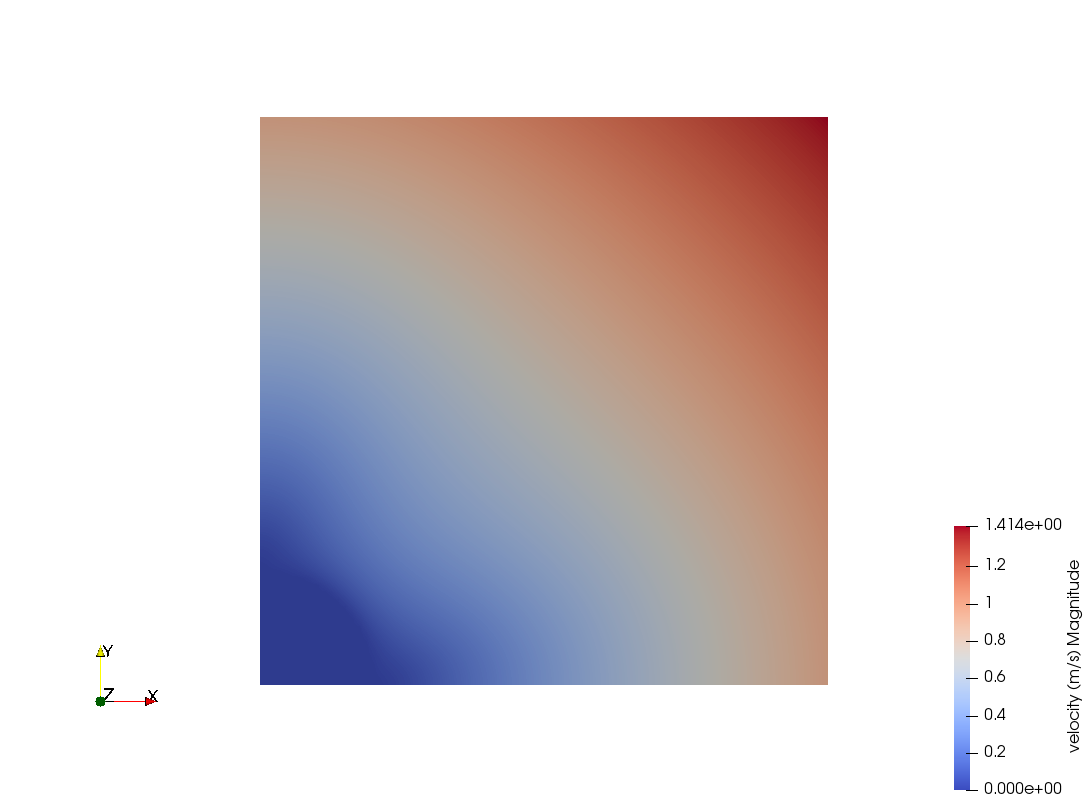
\includegraphics[width=8cm]{./results/benchmark_solvi/vel}
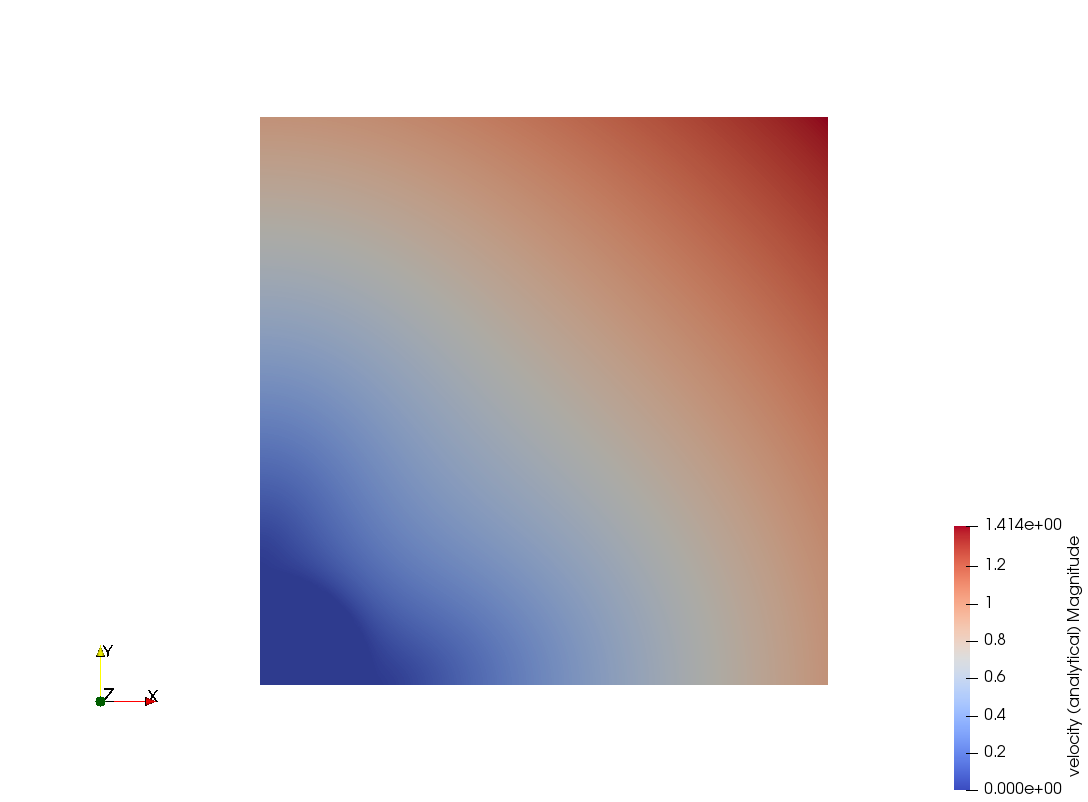
\includegraphics[width=8cm]{./results/benchmark_solvi/vel_analytical}\\
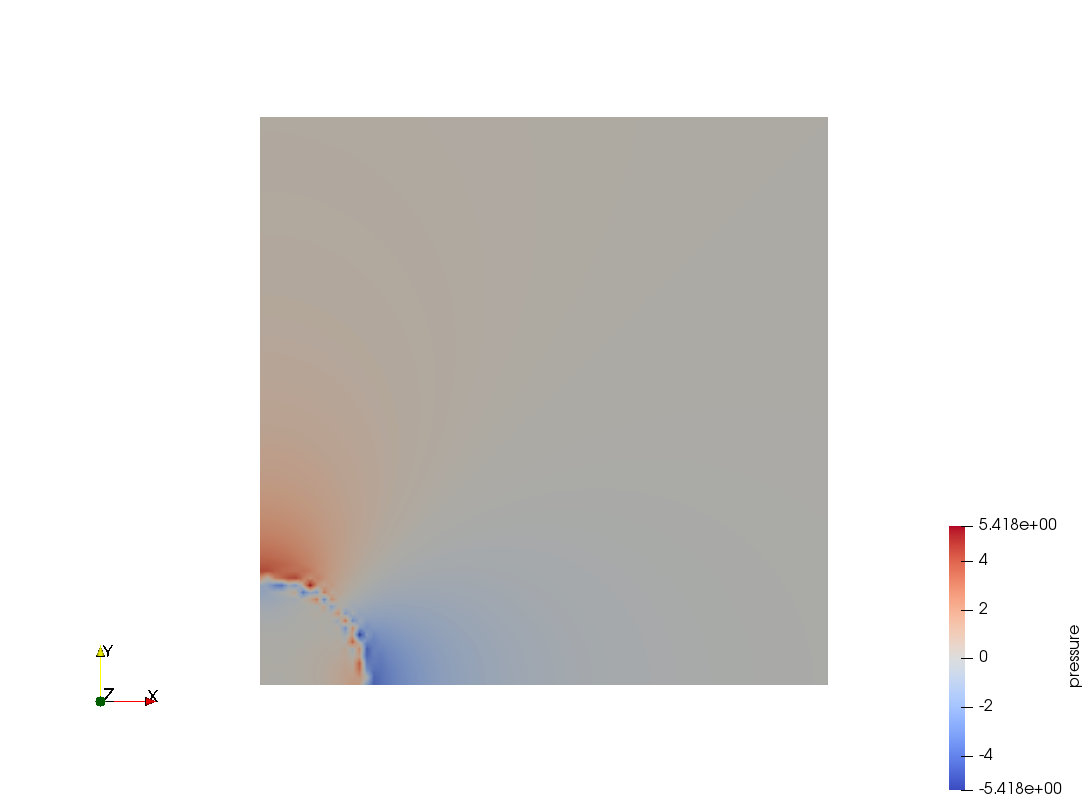
\includegraphics[width=8cm]{./results/benchmark_solvi/press}
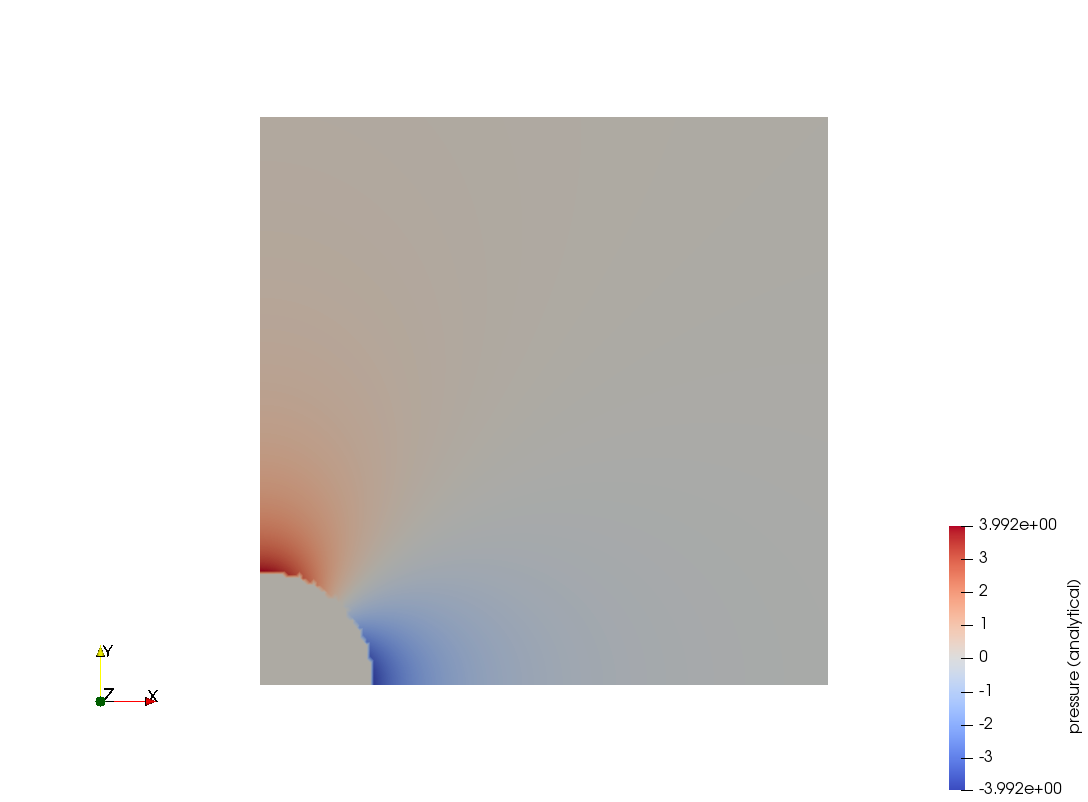
\includegraphics[width=8cm]{./results/benchmark_solvi/press_analytical}\\
{\it Top row: velocity, bottom row: pressure. Left column: computed field, 
right column: analytical solution.}
\end{center}

\begin{center}
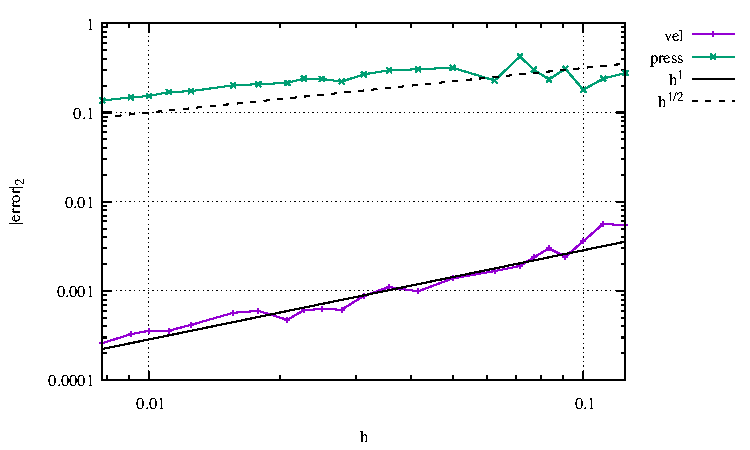
\includegraphics[width=8.7cm]{./results/benchmark_solvi/convergence.pdf}
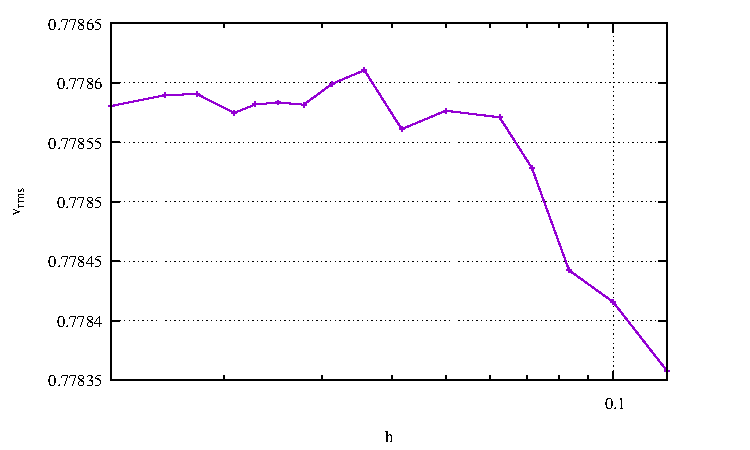
\includegraphics[width=8.7cm]{./results/benchmark_solvi/vrms.pdf}
\end{center}



\subsection{Poiseuille nonlinear}

\subsection{(E)VP experiment gerya 3 mats}

\subsection{darcy? simpson ?}

\subsection{gaussian pulse diffusion in time}






%%%%%%%%%%%%%%%%%%%%%%%%%%%%%%
\newpage
\printbibliography
\end{document}


